\section{Methodology: a Throughput-Safe Coordinator}
\label{sec:method}

\begin{figure*}[!tp]
\centering
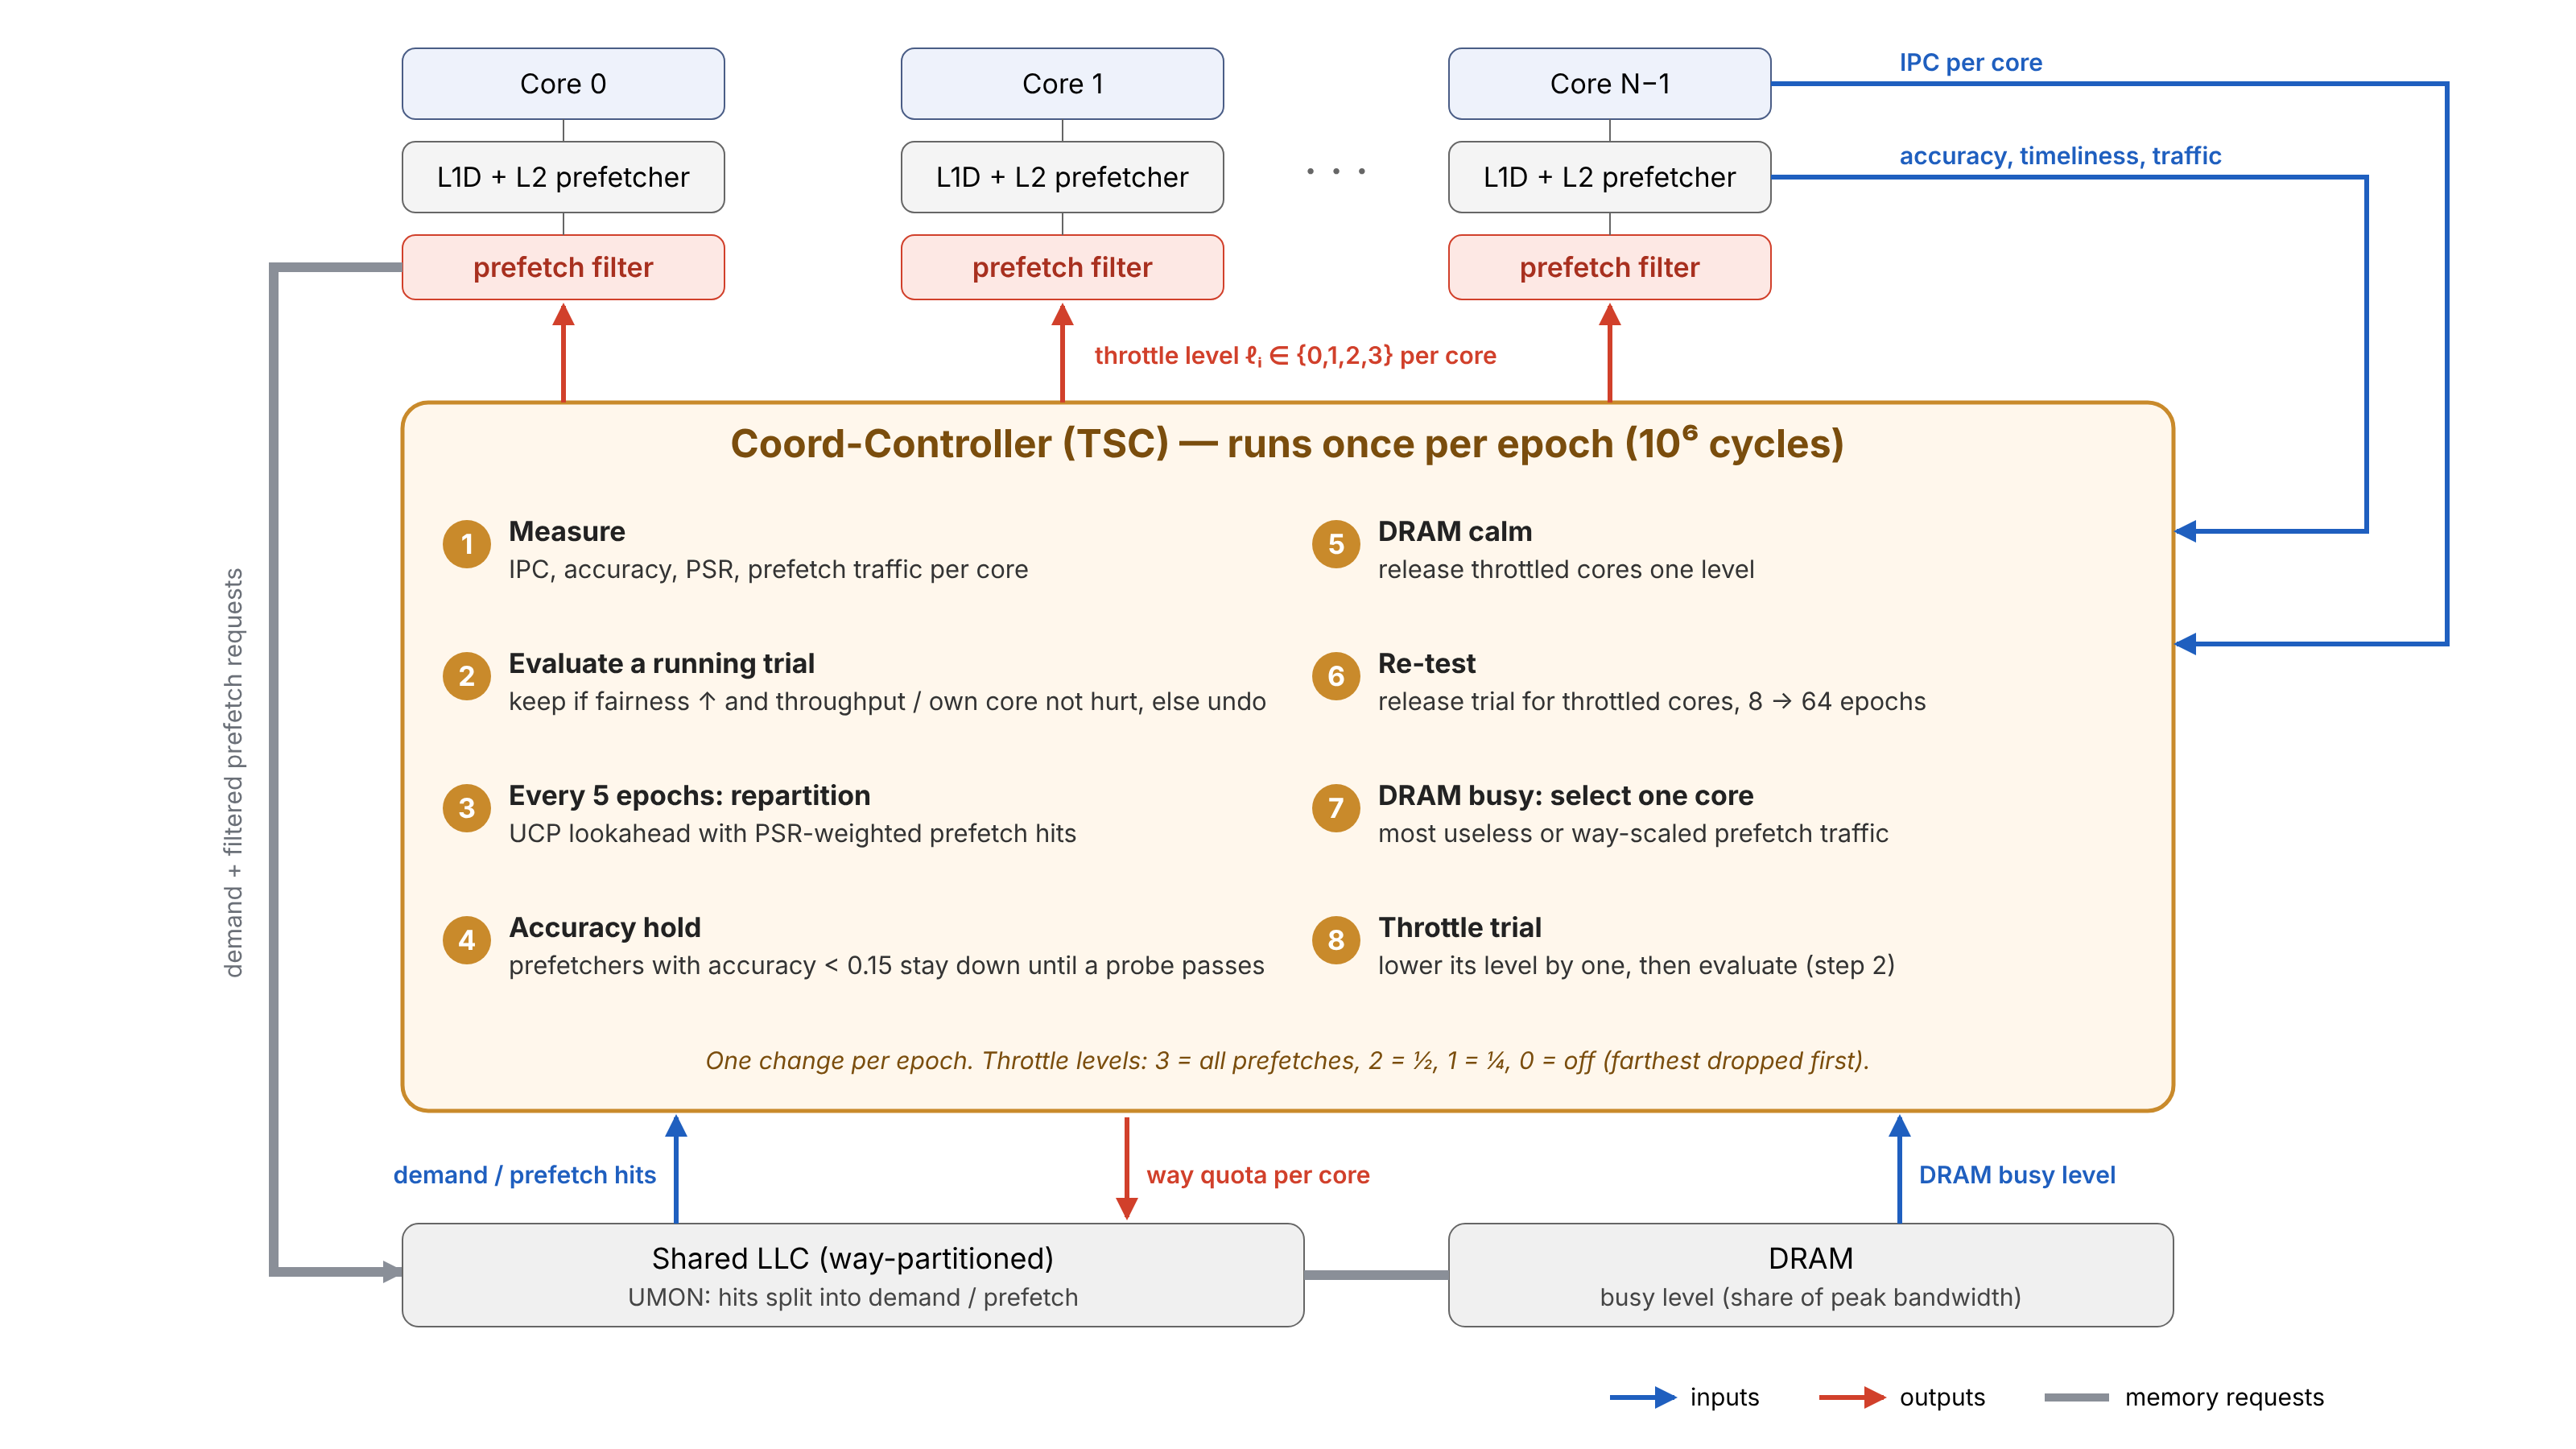
\includegraphics[width=0.92\textwidth]{tsc_overview.png}
\caption{TSC overview.  Once per epoch the coordinator reads per-core IPC, prefetch accuracy, timeliness and
traffic, UCP's demand and prefetch hits and the DRAM busy level (blue), and sets a throttle level per core, applied by
a prefetch filter that drops the farthest requests first, and the per-core LLC way quota (red).}
\label{fig:controller}
\end{figure*}

\Cref{fig:controller} gives an overview.  The coordinator is a small finite-state controller that runs once per epoch
of $10^6$ cycles.  It does not modify the prefetchers, and from UCP it needs only split hit counters and an interface to set the
way quota (\cref{sec:knobs}).  It acts through two interfaces: a \emph{prefetch filter} that lets only part of a core's prefetch requests
through (\cref{sec:knobs}), and the LLC way quota of each core.

\subsection{What the coordinator measures}
\begin{itemize}
  \item \textbf{Per-core prefetch quality} from the private L1D and L2: prefetches filled, \emph{useful} (first
        demand hit on a prefetched block), \emph{late} (demand merged with an in-flight prefetch) and \emph{useless}
        (evicted unused).  Accuracy $a=\text{useful}/(\text{useful}+\text{useless})$, timeliness
        $t=\text{useful}/(\text{useful}+\text{late})$ and the prefetch success rate $\mathit{PSR}=a\cdot t$ are kept as
        exponentially weighted averages.  A request that the prefetch filter drops never reaches the cache, so it is
        never counted as useful, useless or late: the metrics describe only the prefetches that were actually sent.
  \item \textbf{Per-core prefetch DRAM traffic}: LLC prefetch misses per kilo-cycle, and its useless part
        $(1-a)\times$traffic.
  \item \textbf{Per-core IPC} of the epoch, and an exponentially weighted reference IPC.
  \item \textbf{DRAM pressure}: how busy DRAM is, as the share of its peak bandwidth in use, reported in four
        levels numbered 0--3 (below 25\%, 25--50\%, 50--75\%, above 75\%) and averaged over the epoch.  DRAM counts as
        \emph{busy} when this average is above 1.5 (i.e.\ mostly in the upper two levels) and as \emph{calm} when it
        is below.
  \item \textbf{Partition state}: each core's way quota and UCP's sampled shadow-tag hit counters, which we split
        by request type into demand hits $h^d_c[r]$ and prefetch hits $h^p_c[r]$ per LRU position $r$.
\end{itemize}

\subsection{What the coordinator controls}
\label{sec:knobs}
\paragraph{Prefetch filter (farthest requests dropped first)}
Each core has a \emph{throttle level} that sets which share of its prefetch requests is sent:
\begin{center}\footnotesize
\begin{tabular}{lcccc}
\toprule
Throttle level $\ell$ & 3 & 2 & 1 & 0 \\
Share of requests sent $f$ & all & 1/2 & 1/4 & none \\
\bottomrule
\end{tabular}
\end{center}
Level 3, the default, leaves the prefetcher untouched; level 0 switches it off.  \emph{Throttling} a core means lowering its level by one; \emph{releasing} it means raising it by one.  Every
prefetcher sends its requests through one function per cache (\texttt{prefetch\_line}), and the filter sits there.
When a prefetcher is triggered by a demand access, it issues several requests at once, nearest address first (stride,
stream and offset prefetchers all do so); we call these requests a \emph{burst}.  The filter lets the first
share $f$ of each burst through and drops the rest, i.e.\ the farthest, least timely ones.  Example: a prefetcher with
degree 4 issues the lines $+1,+2,+3,+4$ ahead; at level 2 only $+1$ and $+2$ are sent, at level 1 only $+1$.  Because
burst sizes vary, the filter uses the running average burst size $\bar B$ and carries the fraction left over from one
burst to the next, so that a prefetcher issuing one request per trigger is thinned to every second or fourth request.
No prefetcher code is changed.
\paragraph{LLC way quota}
Through five functions (read quota, set quota, enable external control, read and age the split hit counters) the
coordinator replaces UCP's own repartitioning.  We implemented them for UCP only.

\subsection{Prefetch control}

\begin{figure*}[!tp]
\centering
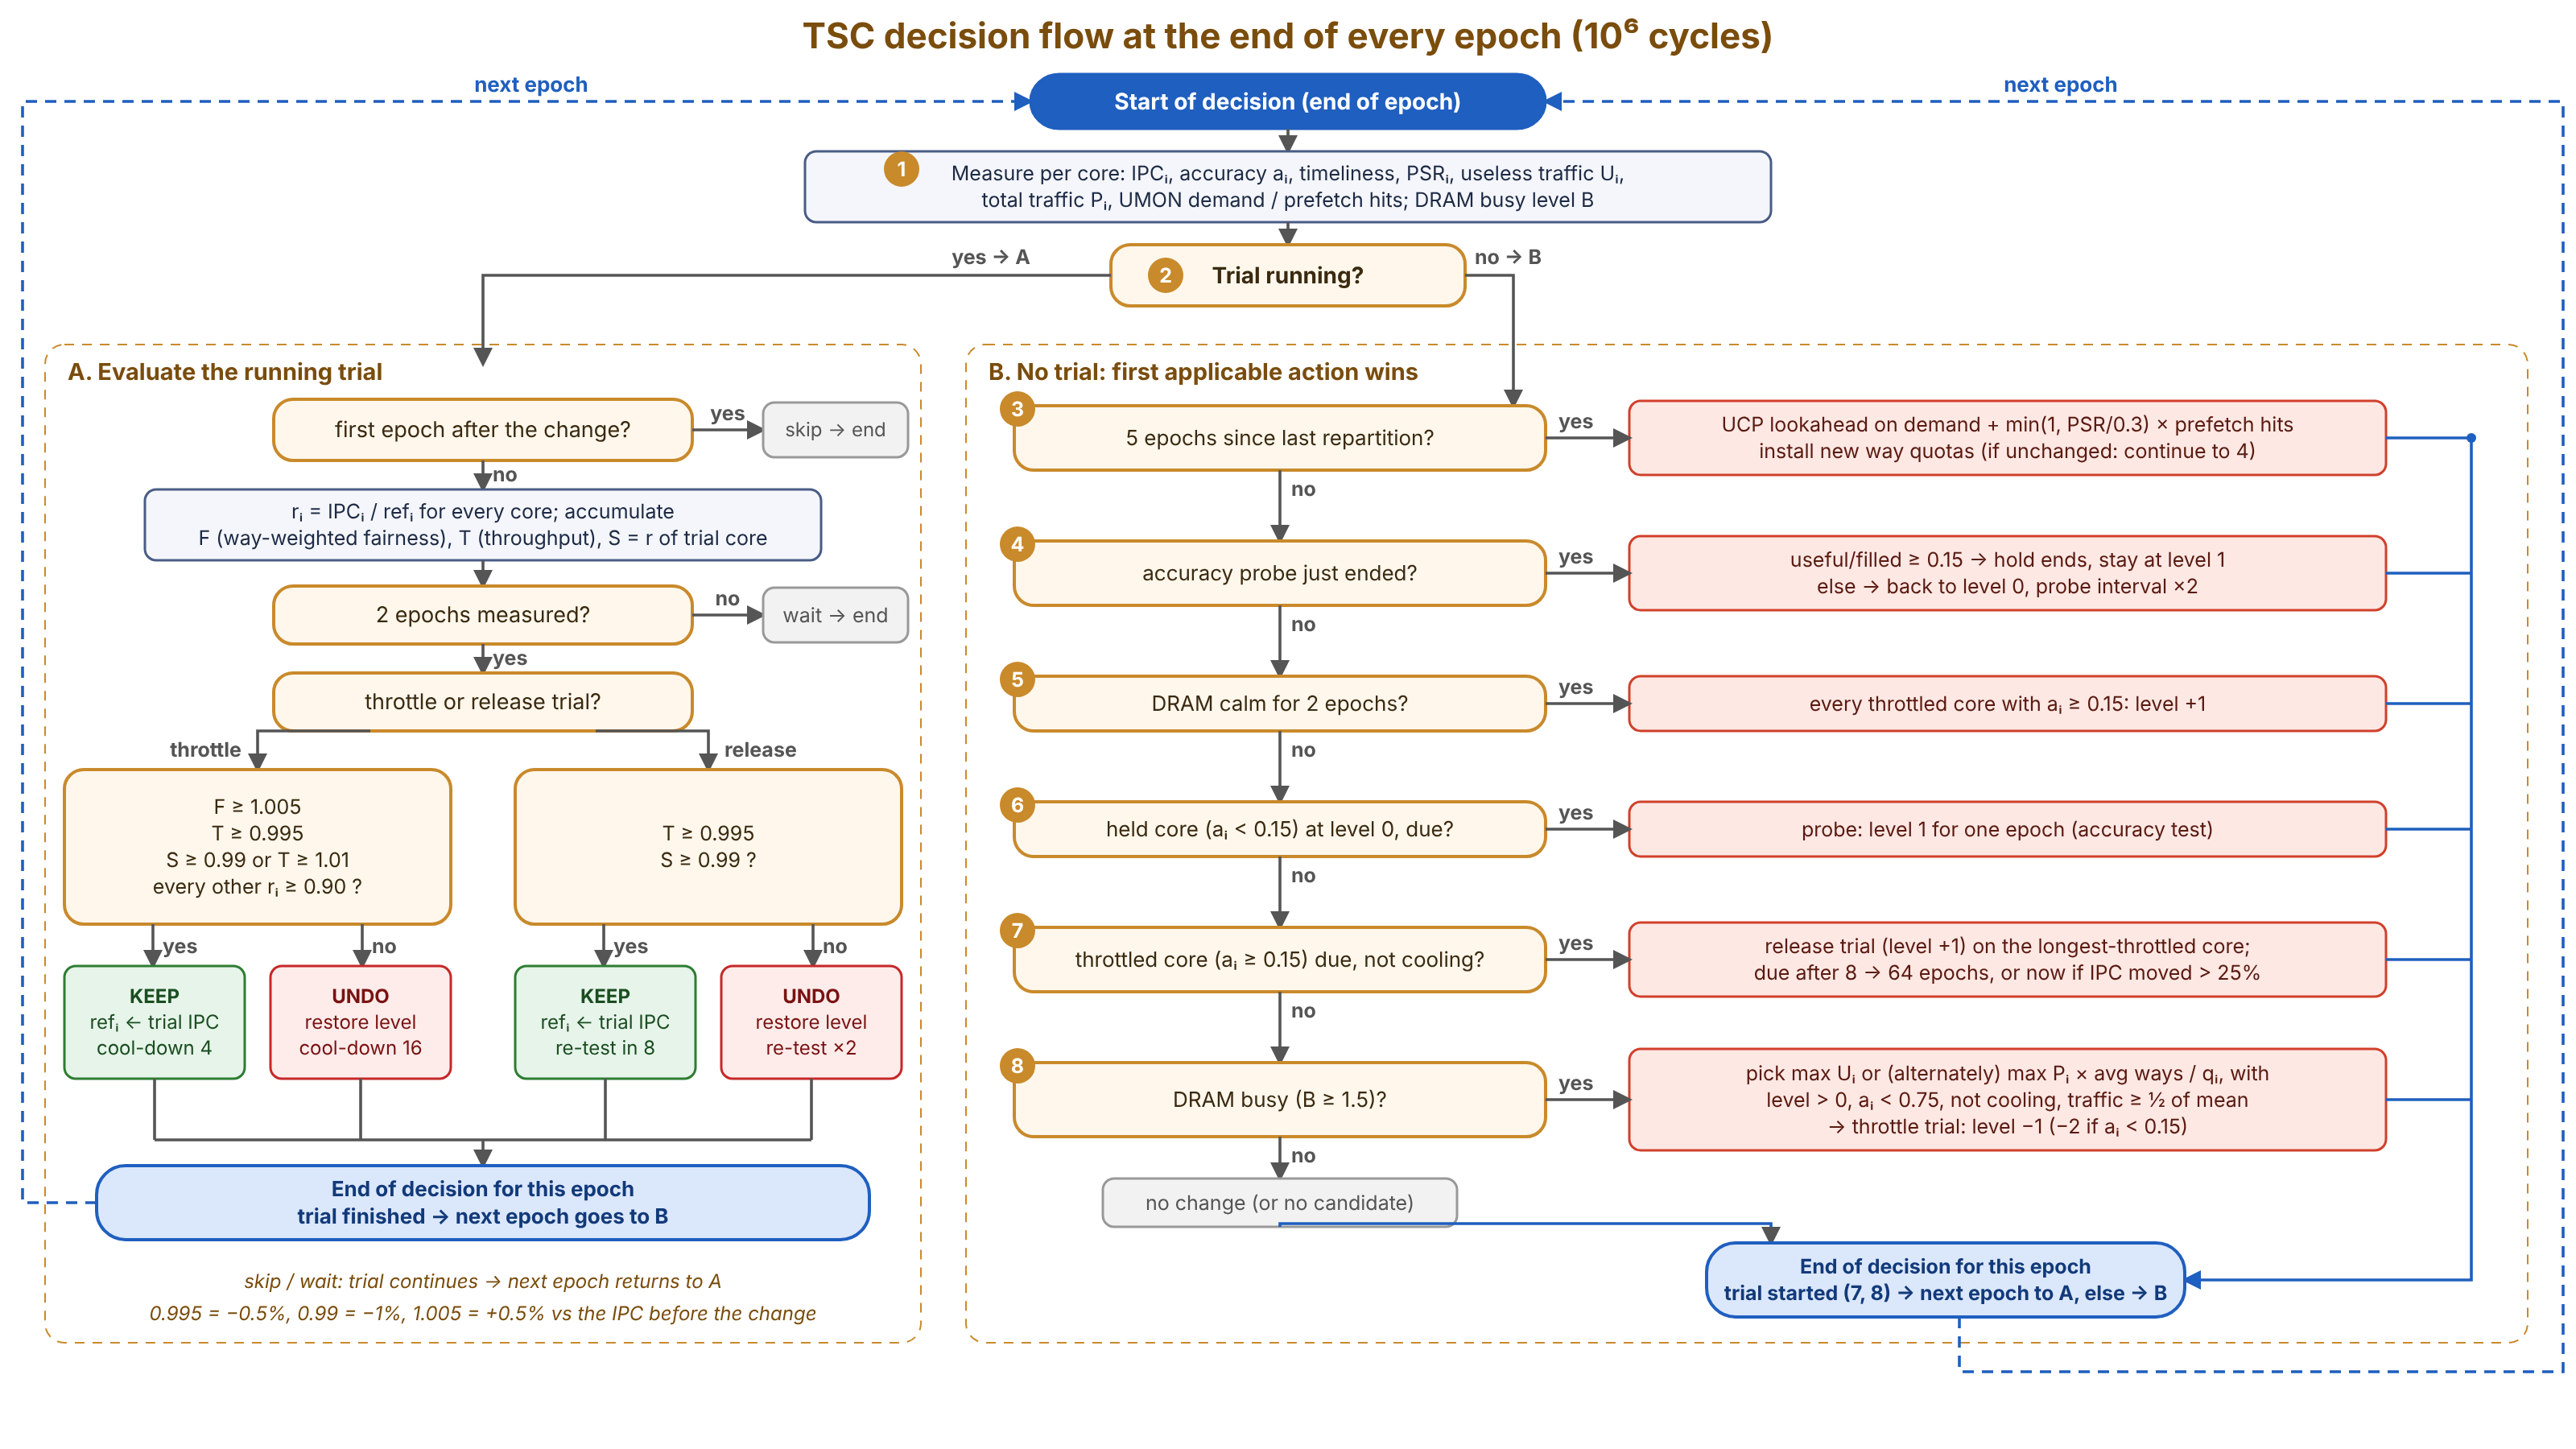
\includegraphics[width=0.95\textwidth]{tsc_flowchart.png}
\caption{TSC decision flow at the end of every epoch.  A running trial is evaluated in A; otherwise the first
applicable action of B is taken.  Every path ends the decision for the epoch; a trial started in B is evaluated in A
in the following epochs, and a finished trial returns control to B.}
\label{fig:flow}
\end{figure*}

\begin{algorithm}[!tp]
\caption{TSC: decision at the end of every epoch.  The functions are in Algorithm~\ref{alg:funcs}, the constants in
\cref{tab:params}.}
\label{alg:epoch}
\small
\DontPrintSemicolon
\SetKwProg{Fn}{Function}{}{end}
\SetKwFunction{FEnd}{EndOfEpoch}\SetKwFunction{FTrial}{Trial}\SetKwFunction{FEval}{Evaluate}
\SetKwFunction{FSel}{SelectCore}\SetKwFunction{FHeld}{Held}\SetKwFunction{FPart}{Repartition}
\SetKwFunction{FProbe}{EndProbe}
\KwIn{per core $i$: $\mathit{IPC}_i$, prefetch accuracy $a_i$ and success rate $\mathit{PSR}_i$, useless and
  total prefetch traffic $U_i$, $P_i$, way quota $q_i$; DRAM busy level $B$}
\KwOut{throttle level $\ell_i\in\{0,1,2,3\}$ and way quota $q_i$ of every core}
\KwData{$\mathit{ref}_i$: reference IPC of core $i$ (its IPC before a change)}
\BlankLine
\Fn{\FEnd{}}{
  \lIf(\tcp*[f]{measure, keep or undo}){a trial is running}{\FEval{}; \Return}
  \lIf(\tcp*[f]{PSR-weighted UCP}){every $E_q$ epochs}{\FPart{}}
  \lIf(\tcp*[f]{held core probed}){a probe has ended}{\FProbe{}; \Return}
  \If(\tcp*[f]{no pressure: give back}){DRAM calm for $C$ epochs}{
    $\ell_i\gets\ell_i+1$ for every throttled $i$ with $\neg$\FHeld{$i$}; \Return
  }
  \lIf(\tcp*[f]{probe}){a held core $i$ at level 0 is due}{$\ell_i\gets1$ for one epoch; \Return}
  \lIf(\tcp*[f]{re-test}){a throttled core $i$ with $\neg$\FHeld{$i$} is due}{\FTrial{$i$, $+1$}; \Return}
  \If(\tcp*[f]{pressure}){$B\ge B_{hi}$}{
    $j\gets$\FSel{}\;
    \lIf{$j\neq\bot$}{\FTrial{$j$, $-2$ \textbf{if} $a_j<a_2$ \textbf{else} $-1$}}
  }
}
\end{algorithm}

\begin{algorithm}[!tp]
\caption{Functions of TSC.}
\label{alg:funcs}
\small
\DontPrintSemicolon
\SetKwProg{Fn}{Function}{}{end}
\SetKwFunction{FTrial}{Trial}\SetKwFunction{FEval}{Evaluate}\SetKwFunction{FFilter}{Filter}
\SetKwFunction{FSel}{SelectCore}\SetKwFunction{FHeld}{Held}\SetKwFunction{FPart}{Repartition}
\SetKwFunction{FProbe}{EndProbe}
\Fn(\tcp*[f]{on every prefetch burst of core $i$}){\FFilter{$i$, burst}}{
  send the nearest share $f(\ell_i)$ of the burst; drop the rest \tcp*[r]{$f=0,\frac14,\frac12,1$}
}
\BlankLine
\Fn{\FHeld{$i$}}{\Return $a_i<a_{\mathit{hold}}$ \tcp*[r]{no release trial, no calm release}}
\BlankLine
\Fn{\FSel{}}{
  $x_i\gets U_i$, or (alternately) $x_i\gets P_i\cdot\bar q/q_i$ \tcp*[r]{useless / way-scaled traffic}
  \Return $\arg\max x_i$ over cores with $\ell_i>0$, $a_i<a_{\mathit{prot}}$, not cooling down\;
}
\BlankLine
\Fn{\FTrial{$j$, $\delta$}}{
  $\ell_j\gets\ell_j+\delta$; skip 1 epoch, then measure $K$ epochs \tcp*[r]{then \FEval}
}
\BlankLine
\Fn{\FEval{}}{
  $r_i\gets\mathit{IPC}_i/\mathit{ref}_i$ for every core\;
  $F\gets$ way-weighted harmonic mean of $r_i$;\ $T\gets$ mean of $r_i$;\ $S\gets r_j$\;
  \eIf(\tcp*[f]{throttle trial}){$\delta<0$}{
    $\mathit{ok}\gets F\ge1+g\ \wedge\ T\ge1-\tau_T\ \wedge\ (S\ge1-\tau_S\ \vee\ T\ge1+\tau_W)$
      $\wedge$ no other $r_i<1-\tau_V$\;
  }(\tcp*[f]{release trial}){
    $\mathit{ok}\gets T\ge1-\tau_T\ \wedge\ S\ge1-\tau_S$\;
  }
  \lIf{$\mathit{ok}$}{$\mathit{ref}_i\gets$ IPC measured in the trial}
  \lElse{$\ell_j\gets\ell_j-\delta$; core $j$ cools down}
}
\BlankLine
\Fn{\FProbe{}}{
  $a\gets$ useful / filled prefetches of the probed core $i$ in the probe epoch\;
  \lIf(\tcp*[f]{hold ends}){$a\ge a_{\mathit{hold}}$}{keep $\ell_i=1$}
  \lElse{$\ell_i\gets0$}
}
\BlankLine
\Fn{\FPart{}}{
  $w_i\gets\min(1,\ \mathit{PSR}_i/\mathit{PSR}_{\mathit{full}})$\;
  $q\gets$ UCP lookahead on demand hits $+\ w_i\cdot$ prefetch hits\;
}
\end{algorithm}

\Cref{fig:flow} shows the decision flow, and Algorithms~\ref{alg:epoch} and~\ref{alg:funcs} give it as pseudocode.  Its design follows directly from the findings of
\cref{sec:problem}.  The central mechanism is the \emph{trial}: the controller never decides from a model whether a
change will help.  It makes one small change (one core, one level), measures its effect on every core for a few
epochs, and keeps the change only if the measurement passes the acceptance test below; otherwise it restores the
previous level.  A \emph{throttle trial} lowers a core's level by one, a \emph{release trial} raises it by one.

\paragraph{One change at a time, measured}
When DRAM is busy, the controller picks the core to throttle by alternating between two rankings.  The first
ranks cores by their \emph{useless} prefetch traffic, i.e.\ prefetched lines that are evicted unused: they use DRAM bandwidth and cache space without
benefit.  The second ranks cores
by their total prefetch traffic, scaled by the average way quota divided by the core's own quota, i.e.\ the cores
that send the most prefetch traffic to DRAM although UCP gives them few ways (UCP's monitors say they gain little
from cache space).  The top candidate gets a throttle trial.  A trial does not score the first epoch after the change and scores the next two.

\paragraph{Throughput-safe acceptance}
Each core $i$ keeps a reference IPC, $\mathit{ref}_i$: an exponentially weighted average of its IPC in the epochs
before the trial.  During the trial its speedup is $r_i=\mathit{IPC}_i/\mathit{ref}_i$.  We compare ratios rather than
raw IPC because the IPC of the cores of a mix differs by up to $15.6\times$ in our 4-core runs (median $5.5\times$).  A sum of IPCs would be dominated by the
fast cores: with IPCs of 1.6 and 0.2, a 5\% speedup of the fast core outweighs a 20\% slowdown of the slow one.  The ratio counts every core's relative change equally, as the weighted speedup does.
From the ratios the controller computes
\[
  T = \frac{1}{N}\sum_{i=1}^{N} r_i, \qquad
  F = \frac{\sum_i w_i}{\sum_i w_i/r_i},
\]
where $w_i = 1 + q_i/\bar q$, with $q_i$ the way quota of core $i$ and $\bar q$ the average quota (16 ways divided
by the number of cores).  $T$ and $F$ are computed for each of the two scored epochs and averaged.
$T$, the arithmetic mean, is the trial's throughput (normalised weighted speedup).  $F$, the harmonic mean, is
dominated by the smallest ratios, so it rises when a slowed-down core recovers; we call it the \emph{way-weighted fairness}.  Weighting it by
the way quota gives more weight to the cores to which UCP gives more ways; with IPCP, the casualties are mostly
cache-sensitive cores (\cref{fig:interaction}).  A throttle trial
is kept only if (i)~the way-weighted fairness $F$ rises by at least the gain $g=0.5\%$, (ii)~$T$ drops by at most 0.5\%, (iii)~the throttled
core itself loses at most 1\% unless $T$ rises by at least 1\%, and (iv)~no other core loses more than 10\%.  A
release trial is kept if $T$ and the released core do not lose more than 0.5\% and 1\%.  Rule~(iii) is the main difference to FDT.  On 4 cores at 2.4\,GB/s per core, the cores that the independent run
speeds up by at least 1.3$\times$ are throttled 39\% (IPCP) and 9\% (Pythia) of the time under \vthree{}, against
90\% and 82\% under FDT, and end up $+2.4\%$ and $-0.4\%$ instead of $-13.7\%$ and $-12.0\%$.

\paragraph{Gradual, periodically re-justified throttling}
Prefetching is the default.  A level is never removed or restored in one jump: each level is its own trial.  Every
throttled core is \emph{revalidated}: after 8 epochs it gets a release trial, which is kept unless throughput or the
core itself suffers.  A rejected revalidation doubles the interval, up to 64 epochs, and a phase change (the core's IPC
moved by more than 25\%) resets it.  When DRAM is calm for two epochs, every throttled core gets one level back.

\paragraph{Accuracy hold}
A throttled core whose accuracy is below 0.15 receives no release trial and is not released when DRAM is calm.
On 4 cores at 2.4\,GB/s per core, none of the 26 cores with an accuracy below 0.15 runs more than 2\% faster with both
mechanisms than with neither (at 9.6\,GB/s, 4 of 26 do; \cref{sec:limits}).  Adding the hold raises throughput from
4.6\% to 7.1\% (IPCP, \cref{tab:final4}).
At level 0 it issues no prefetches, so its accuracy is probed: one unjudged epoch at level 1, judged by
useful/filled prefetches of that epoch (both counted immediately, unlike evictions); only an accuracy of at least
0.15 ends the hold.

\subsection{Partition control}
Every five epochs (UCP's own interval) the coordinator computes the allocation with UCP's lookahead algorithm on the
utility
\[
  u_c[r] = h^d_c[r] + w_c\, h^p_c[r], \qquad w_c=\min\!\left(1,\ \mathit{PSR}_c/0.3\right),
\]
and installs it directly, without a trial.  A core whose prefetches are accurate and timely ($\mathit{PSR}\ge0.3$)
keeps exactly the ways UCP would give it, since UCP counts demand and prefetch hits alike; for a core with
$\mathit{PSR}<0.3$ the prefetch hits count only in proportion to its PSR.  The coordination thus works in both
directions: prefetch quality sets the partition's utility, and the way quota enters the throttling through the
way-weighted fairness $F$ and the way-scaled traffic ranking.

\subsection{Parameters and cost}

\begin{table}[!htbp]
\centering
\caption{Coordinator parameters (sensitivity in \cref{sec:sweep}).}
\label{tab:params}
\footnotesize
\resizebox{\columnwidth}{!}{\begin{tabular}{llr}
\toprule
Symbol & Meaning & Value \\
\midrule
$N$, $Q$ & cores, LLC ways & 4 or 8, 16 \\
-- & epoch length & $10^6$ cycles \\
$E_q$ & partition period & 5 epochs \\
$K$ & scored epochs per trial (after 1 skipped) & 2 \\
$\alpha$ & EWMA weight of the reference IPC & 0.3 \\
$B_{hi}$ & DRAM busy threshold (level 0--3) & 1.5 \\
$C$ & calm epochs before a release & 2 \\
$g$ & way-weighted fairness gain & 0.5\% \\
$\tau_T$ & throughput budget & 0.5\% \\
$\tau_S$ & own-core budget & 1\% \\
$\tau_W$ & throughput gain that overrides $\tau_S$ & 1\% \\
$\tau_V$ & victim guard (any other core) & 10\% \\
$a_{\mathit{prot}}$, $a_2$, $a_{\mathit{hold}}$ & protect / two-level drop / hold accuracy & 0.75 / 0.15 / 0.15 \\
$\sigma$ & minimum share of the mean traffic to be a candidate & 0.5 \\
$R_0$, $R_{\max}$ & revalidation interval, back-off limit & 8, 64 epochs \\
$\varphi$ & phase change (IPC change since last level change) & 25\% \\
$c_{\mathit{keep}}$, $c_{\mathit{rev}}$ & cool-down after a kept / reverted trial & 4, 16 epochs \\
$\mathit{PSR}_{\mathit{full}}$ & PSR for full prefetch credit in the UMON & 0.3 \\
\bottomrule
\end{tabular}}
\end{table}

\Cref{tab:params} lists the parameters.  The state is small: per core a 2-bit level, five 16-bit averages
(accuracy, timeliness, useless and total traffic, reference IPC), three 8-bit timers and the burst state of the filter
(about 4 bytes per cache), i.e.\ roughly 20 bytes per core, plus 16 additional prefetch-hit counters per core in the
UMON (64 bytes per core).  The decision logic runs once per epoch; the lookahead allocation runs every five epochs on
$N\times16$ counters, as in UCP.
